\subsection{Einleitung}
Das mittelständige Unternehmen ist in den Bereichen Maschinenbau, Reparaturen und Instandsetzungen sowie Verkauf und Vermietung tätig. Die Produkte des Verkaufs und der Vermietung sind hochwertige Elektromaschinen sowie Werkzeuge und Verbrauchsmaterialien. Desweiteren werden Instandhaltungs- und Reparaturaufträge für Maschinen sowie Spezialanfertigung im Bereich Maschinenbau angeboten. Die Kundschaft besteht überwiegend aus selbstständigen Handwerkern, kleineren Betrieben und Angehörigen aus Land- und Forstwirtschaft. \cite{einleitung1}
\subsection{Ist-Zustand}
Die Warenabgabe im Verkauf und der Vermietung erfolgt in einem Ladengeschäft mittels handgeschriebener Rechnungen und Aufträge. Im nächsten Schritt werden die Aufträge und Rechnungen zur weiteren Verwendung in das bestehende MS-DOS-System wiederholt händisch übertragen. Im darauffolgenden Schritt werden die handgeschriebenen Belege an die Buchhaltungsabteilung zur Prüfung des Rechnungseingangs und Rechnungsausgangs sowie an die Fertigungsabteilung zur Auftragsbearbeitung weitergereicht. \textbf{Screenshots vorhanden vom DOS System?} \cite{einleitung1}
\begin{figure}[!ht]
    \centering
    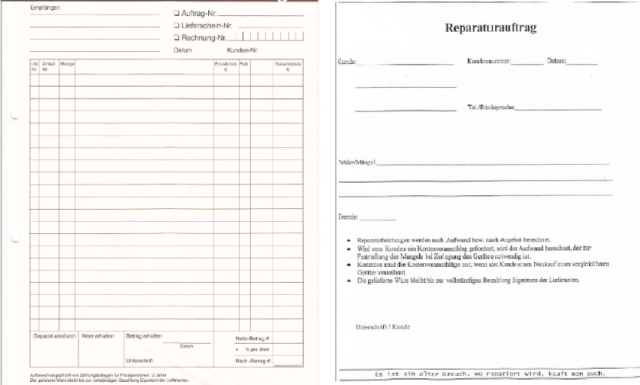
\includegraphics{rechnungReparaturAlt2.png}
    \caption[Muster Rechnungsvordruck und Reparaturauftrag]{\small{Muster eines Rechnungsvordruck (li.) und Reparaturauftrag (re.) \cite{einleitung1}}}
    \label{fig:4}
\end{figure}
\subsection{Ziele}
Das Hauptziel der Umstellung ist die Ablösung des bestehenden Altsystems und der daraus resultierenden Vereinfachung und Beschleunigung der Geschäftsprozesse. Die Entlastung der Mitarbeiter sowie die Kostenreduzierung und Effizienzsteigerung sind weitere Ziele. Das Ziel der personalisierten Warenabgabe ist der eindeutige Nachweis über die erbrachten Lieferungen und Leistungen sowie die rechtliche Absicherung gegenüber Dritten. Im Bereich Umsetzung werde ich hauptsächlich auf die personalisierte Warenabgabe mittels digitaler Signatur eingehen. \cite{einleitung1}